\chapter{Install}


\section{Basic requirements}


To install this network, you will need a few devices.
First you will need a computer with a linux OS (the development of the project was done on Ubuntu). But you also need a few devices:
\begin{itemize}
	\item routers that support openwrt (I used GL-AR150 and GL-AR750)
	\item RFD900+ with serial to usb adaptor
\end{itemize}

Here is a list of all the package you need on your Linux machine:
\begin{itemize}
	\item gcc 
	\item binutils
	\item bzip2
	\item flex
	\item python
	\item perl
	\item make
	\item find
	\item grep
	\item diff
	\item unzip
	\item gawk
	\item getopt
	\item subversion
	\item libz-dev
	\item libc headers
\end{itemize}



\section{Network setup}


For this part, i will suppose you are using openwrt or Lede routers that support wireless communication.

First let's start by looking at the result we want. 
We have many remote sites and 1 main site. The main site is a Wi-Fi access to all the remote sites and it will be the main part of the configuration.

For this site I used GL-AR750. 
We will have a main router and a "`slave"' router.
The main router will have a DHCP server and he will therefore give the addresses to all the devices.

The slave router will connect to the main router and act as a Wi-Fi bridge. 
The GL-AR750 does not allow us to "`physically"' bridge our local network (Wi-Fi + ethernet ports) and the connection with the main router. That's why we are going to use a packet called relayd that will allow us to simulate that bridge.

So the general steps are:
\begin{itemize}
	\item Configure the main router by:
		\subitem creating a Wi-Fi LAN 
		\subitem configuring fixed ip addresses for the small remote routers
	\item Configuring the slave router by:
		\subitem installing relayd
\end{itemize} 

We want to create a network like the one below:
\begin{figure}[H]
\begin{center}
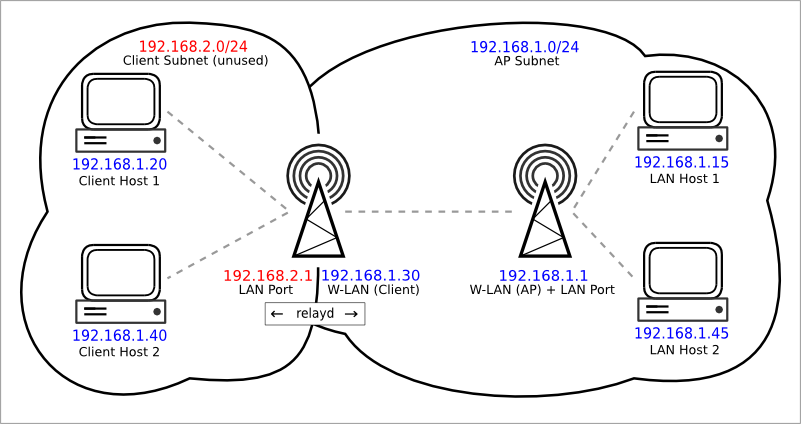
\includegraphics[width=\columnwidth]{image/802-11-routed-relay.png}%
\caption{Bridge network using relayd (source:https://wiki.openwrt.org/doc/recipes/relayclient)}%
\label{figure:interface3}%-
\end{center}
\end{figure}


\subsection{Configuration of the main router}

All the configuration is done through the web interface at the address: http:\/\/192.168.8.1\/cgi-bin\/luci.
The IP address can change depending on the router you have. If you are using routers from GL-INET such as GL-AR750, it should be 192.168.8.1. Otherwise, you need to look at the documentation of your router.


\hfill \break \underline{\large{\textbf{Creating the Wi-Fi LAN}}}

The first we want to do is to create the Wi-Fi and setup the LAN. 
So we first go to the Network $\rightarrow$ wireless tab.
On this tab you should have two pre-configure networks (if you are using a GL-AR750).


We can remove all the networks here and we are going to create a new one. Once created, we will get the following page:
%figure
\begin{figure}[H]
\begin{center}
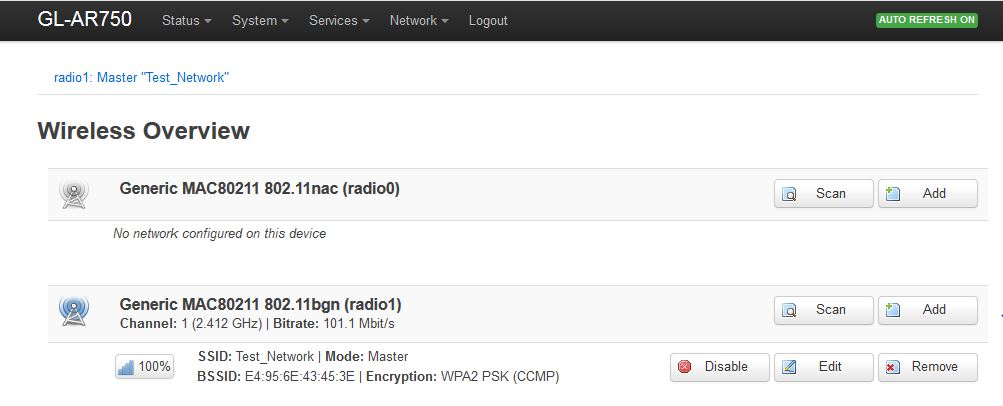
\includegraphics[width=\columnwidth]{image/wireless1.jpg}%
\caption{Wi-Fi network created}%
\label{figure:wireless1}%-
\end{center}
\end{figure}



To create this network, you click on add. It will open a new page that you need to configure as such:
%figure
\begin{figure}[H]
\begin{center}
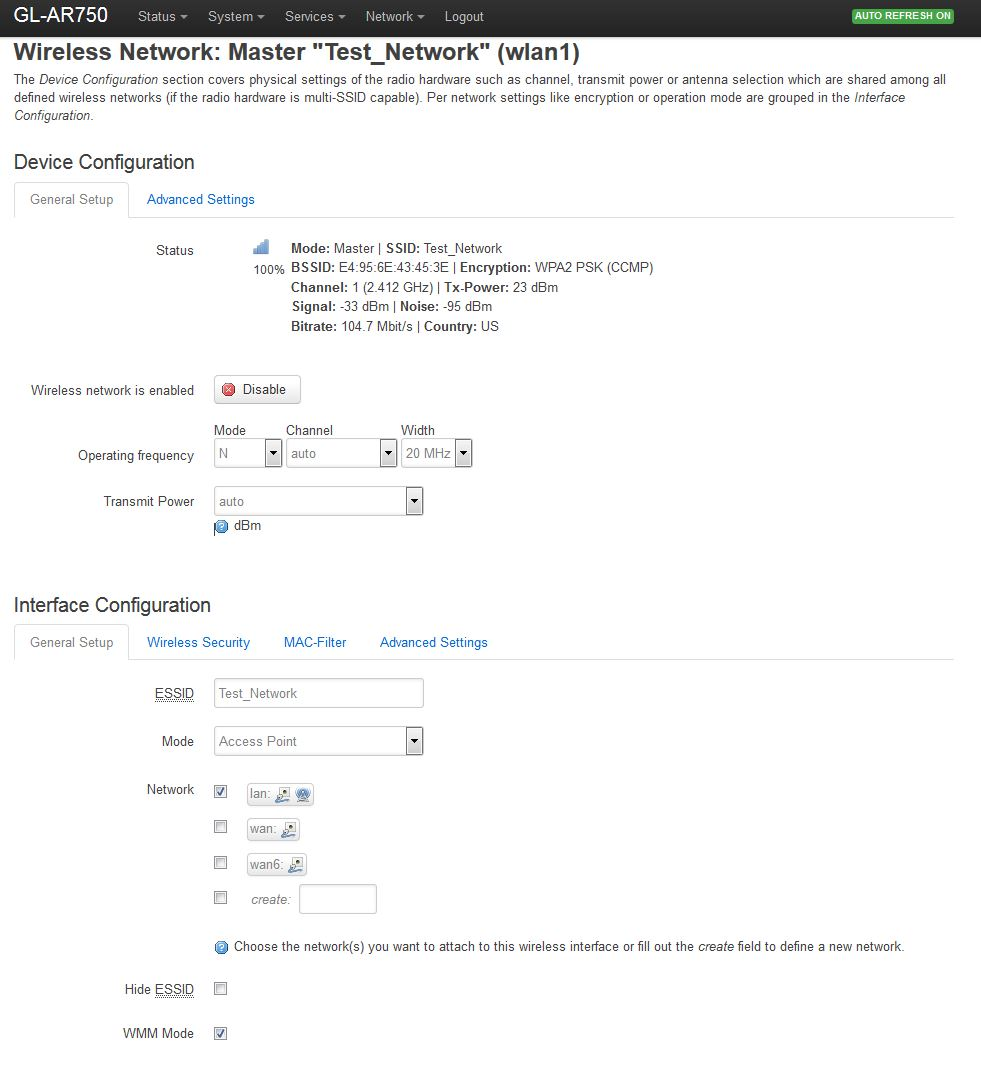
\includegraphics[width=\columnwidth]{image/wireless2.jpg}%
\caption{General configuration of the Wi-Fi network}%
\label{figure:wireless2}%-
\end{center}
\end{figure}


On the device configuration, we want the router to automatically choose the channel.
On the interface configuration, we want to:
\begin{itemize}
	\item choose an SSID
	\item choose the mode Access Point
	\item the network is lan
\end{itemize}

We now go on the wireless security tab and set it up like below:
%figure
\begin{figure}[H]
\begin{center}
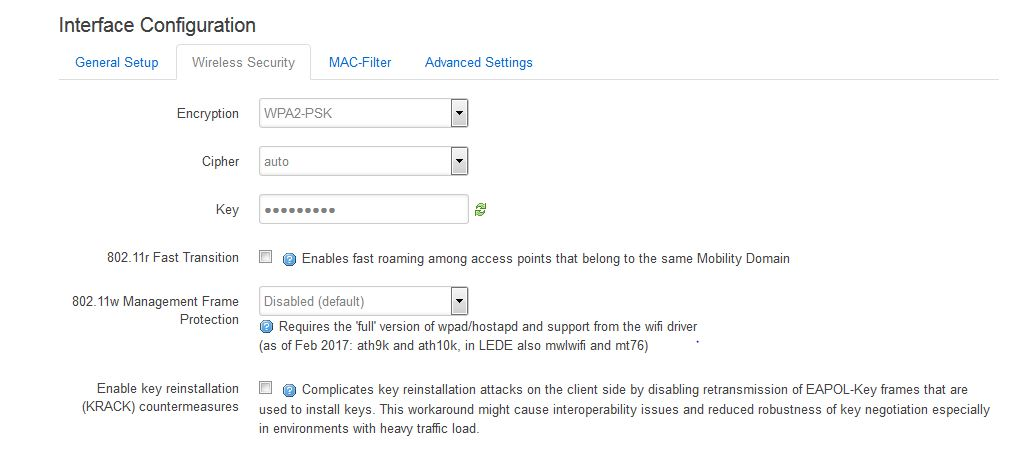
\includegraphics[width=\columnwidth]{image/wireless3.jpg}%
\caption{Security parameters}%
\label{figure:wireless3}%-
\end{center}
\end{figure}
Here we want to create

We are now done and can save the changes. We have successfully created a new Wi-Fi network. We can move on the DHCP setup.

\hfill \break \underline{\large{\textbf{Static DHCP lease}}}

For that part, we go to the Network $\rightarrow$ DHCP and DNS tab. We go at the bottom of the new page to find the section "Static Leases".
In this section, we can add static DHCP leases. We configure it like that:
%figure
\begin{figure}[H]
\begin{center}
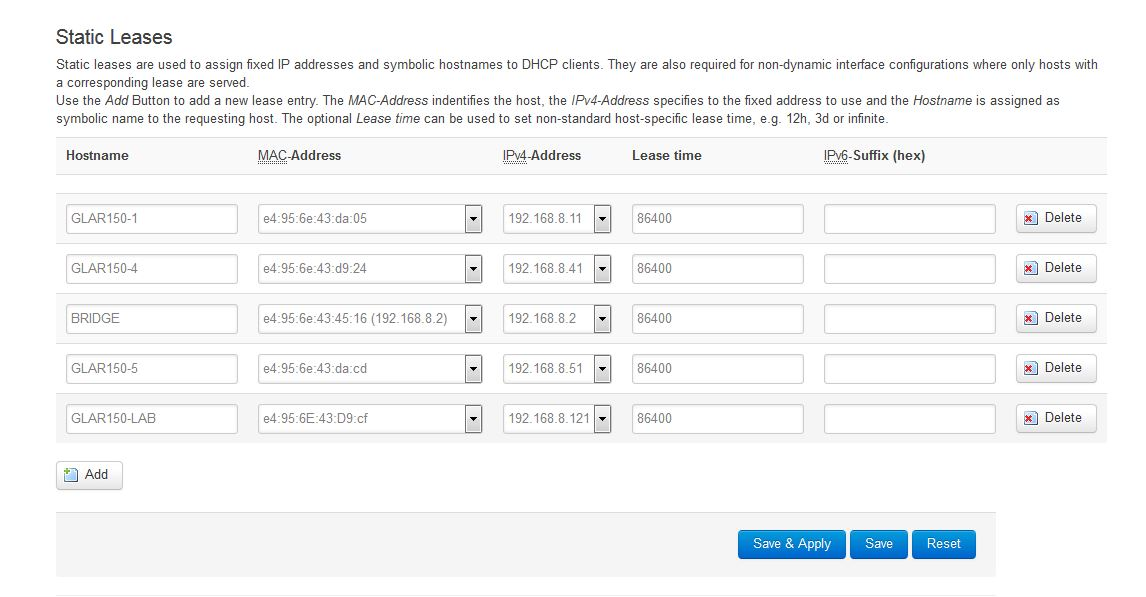
\includegraphics[width=\columnwidth]{image/DHCP1.jpg}%
\caption{DHCP static leases }%
\label{figure:DHCP1}%-
\end{center}
\end{figure}


Pressing the button add, we can manually add a static lease. Static lease work using the mac address of the device. 

\subsection{slave router configuration}

The slave router is a bit more complex to install. Indeed with a GL-AR750, by default, it is not possible to bridge a Wi-Fi Network to another Wi-Fi network. Thankfully, a linux package lets you simulate this behaviour. This package is relayd.
So we are going to install and setup relayd.

\hfill \break \underline{\large{\textbf{Installation of relayd}}}

To install relayd, we need to give the router an access to internet. To do that, you can simply plug the WLAN Ethernet interface to your internet access point or you can plug it to your computer and make your computer share its connection.

Then you connect to the router with ssh (on windows you can use putty).
We want to install two packages:
\begin{itemize}
	\item relayd
	\item luci-proto-relay
\end{itemize}

For that you can use the command:
\begin{lstlisting}
	opkg install package
\end{lstlisting}

Once the package installed we are going to set it up through the web interface. We can use this tutorial to help us:https://wiki.openwrt.org/doc/recipes/relayclient.

We can connect to the same web page as earlier (but for the slave router):http://192.168.9.1/cgi-bin/luci/
The global steps are the following:
\begin{itemize}
	\item Join the network of the main router created earlier
	\item Set up the Wi-Fi interface
	\item create the bridge interface with relayd
	\item update the LAN interface
	\item Set up the firewall
\end{itemize}

\hfill \break \underline{\textbf{Joining the network of the main router}}

The slave server is going to be a client of the main router. For that we head up to Network $\rightarrow$ wireless. We remove the existing network and we create a new one:

\begin{figure}[H]
\begin{center}
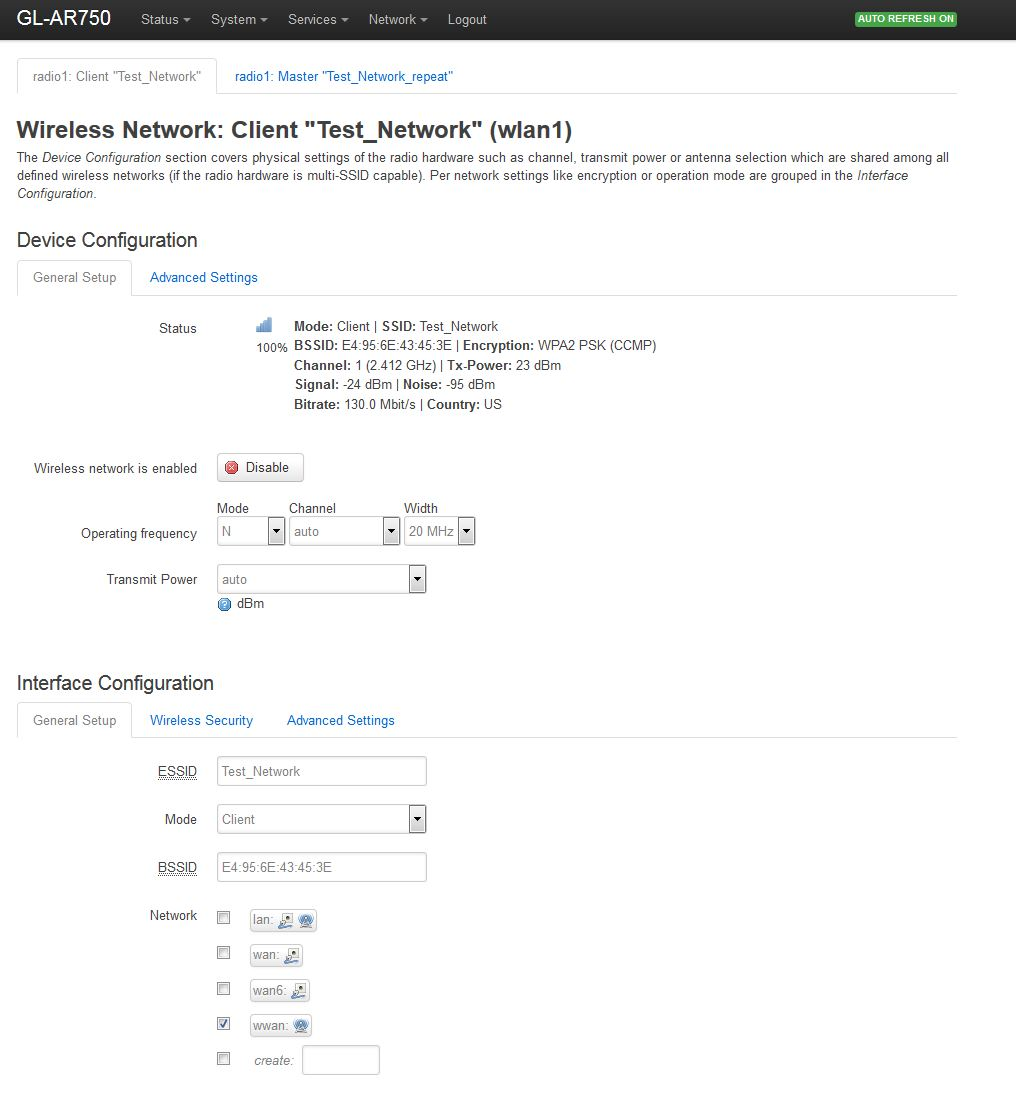
\includegraphics[width=\columnwidth]{image/wireless4.jpg}%
\caption{Joining the main router network}%
\label{figure:wireless4}%-
\end{center}
\end{figure}

We configure this network in the same way as the network on the main router. The only difference is the mode and the network. Instead of choosing access point, we choose Client. For the network, we create a new one and call it wwan (it will not exist at first, you need to enter it in the create field). We save and apply theses changes.

\hfill \break \underline{\textbf{Create a new Wi-Fi network}}

We are going to create a new Wi-Fi network. We go to the Network $\rightarrow$ interfaces and click on edit for the "WWAN" interface.
In the "General Setup" we change the protocol to "DHCP Client" (this means that the slave router will automatically get its IP address from the main router).



\hfill \break \underline{\textbf{Create the bridge interface}}

We go back to the Network $\rightarrow$ interface tab. Here, we create a new interface by clicking "Add new interface".
We set it up like that:

\begin{figure}[H]
\begin{center}
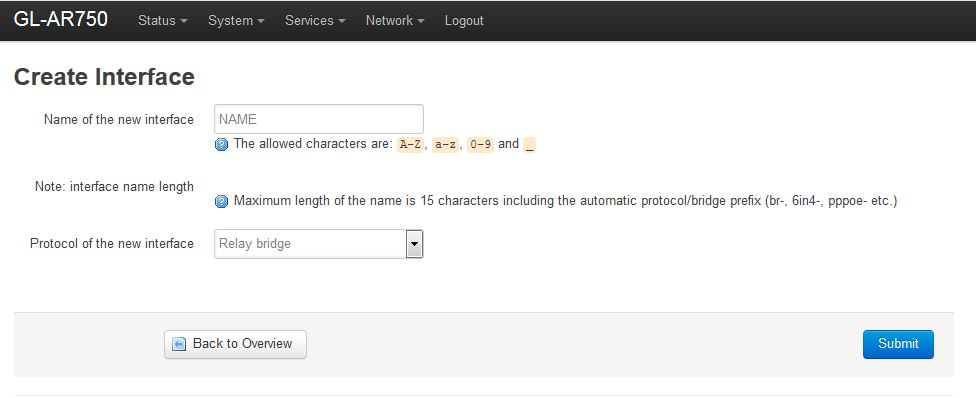
\includegraphics[width=\columnwidth]{image/interface2.jpg}%
\caption{Creation of the bridge interface}%
\label{figure:interface2}%-
\end{center}
\end{figure}

You can choose the name you want for this new interface. I personally chose REPEATER\_TEST. The important setting is protocol. We want to choose "Relay bridge". This option will only appear if we have installed the package luci-proto-relay and the package relayd.
We validate the creation by submitting it.

Now we go back to the interfaces. A new interface, bearing the name we chose, is present. We are going to edit it like the figure below:
\begin{figure}[H]
\begin{center}
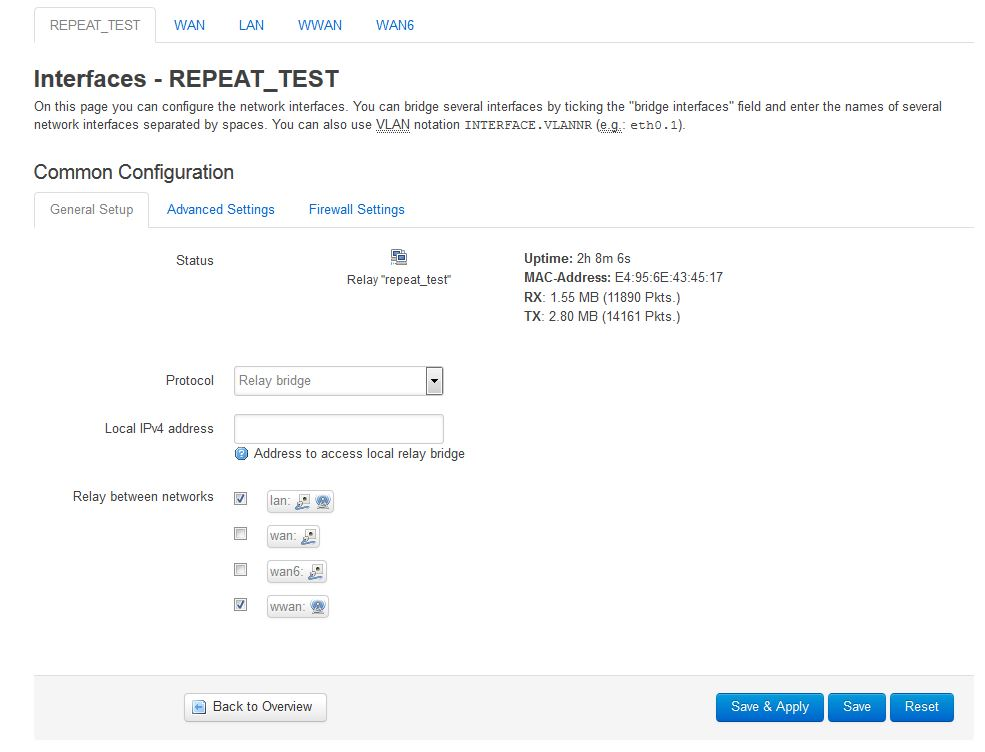
\includegraphics[width=\columnwidth]{image/interface3.jpg}%
\caption{General set up the bridge interface}%
\label{figure:interface3}%-
\end{center}
\end{figure}
Here we want to choose the network we want to bridge. We want to bridge the LAN network to the WWAN one. Therefore, every client that connect to the LAN of this router will be bridged to the WWAN network and therefore the main router.

In the "Advanced Settings", we want to make sure that "Forward DHCP traffic" is ticked (it should be ticked by default):
\begin{figure}[H]
\begin{center}
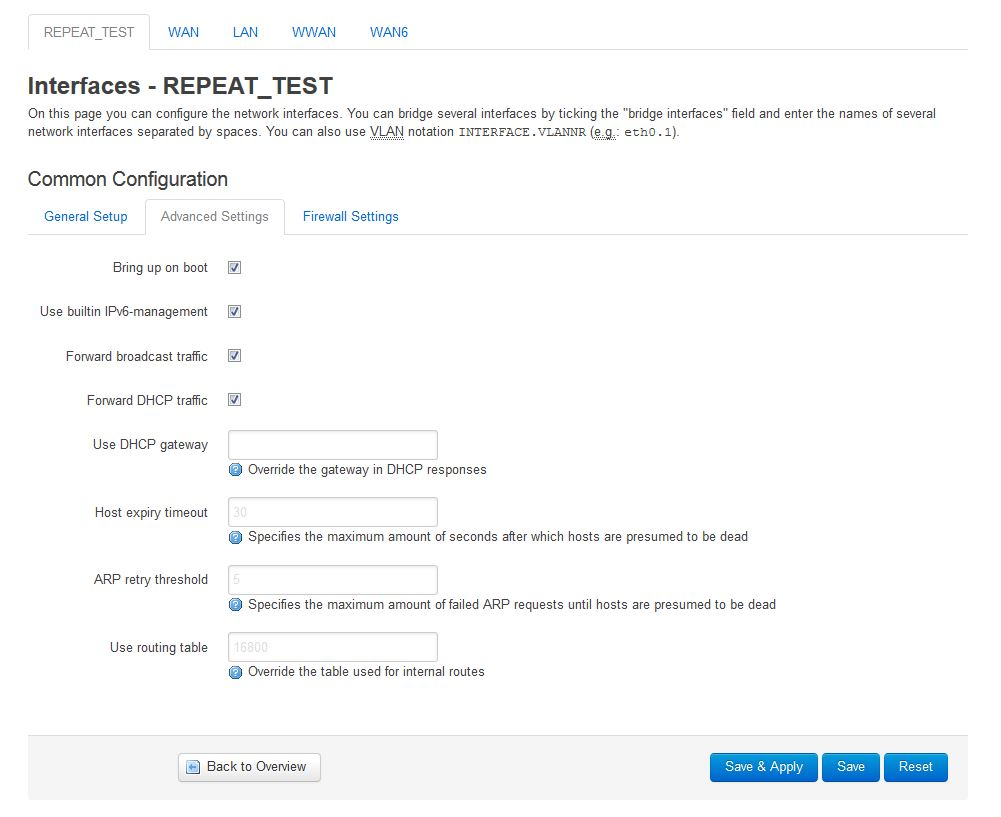
\includegraphics[width=\columnwidth]{image/interface4.jpg}%
\caption{Advanced settings of the bridge interface}%
\label{figure:interface4}%-
\end{center}
\end{figure}

We are now done with the bridge interface and we need to modify the LAN interface.



\hfill \break \underline{\textbf{Update the LAN interface}}

We go to the Network $\rightarrow$ Interfaces tab. We want to edit the LAN interface like below:
\begin{figure}[H]
\begin{center}
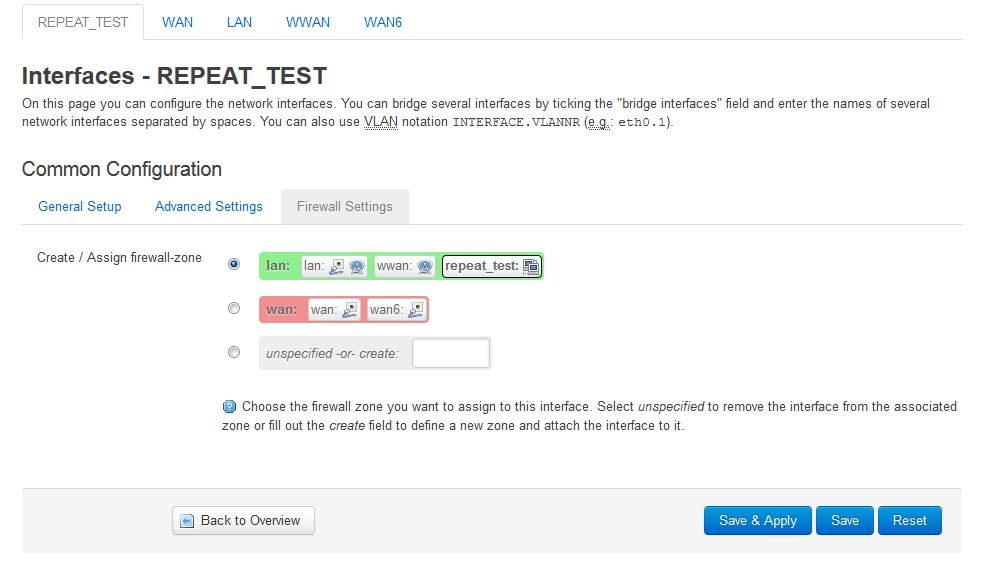
\includegraphics[width=\columnwidth]{image/interface5.jpg}%
\caption{General settings of the LAN interface}%
\label{figure:interface5}%-
\end{center}
\end{figure} 

Here we are going to use a fix address and no DHCP. We want a different address than the one used by the main router.





\hfill \break \underline{\textbf{Set up the firewall}}



\hfill \break \underline{\textbf{Set up the firewall}}


\subsection{remote router configuration}

The configuration of the remote router is quite easy. It has 2 steps:
\begin{itemize}
	\item modify the traffic rules of the router
	\item modify the configuration of the LAN interface
\end{itemize}

\section{Software installation}

The software part consist at downloading the sources files and installing them. We want to install 2 differents part:
\begin{itemize}
	\item a client part for linux
	\item a server part for openwrt
\end{itemize}

\subsection{client installation}

The client part is pretty straightforward as you just need to use the makefile by tiping:
\begin{lstlisting}[language=bash]
	###: make client
\end{lstlisting}
It will create two executable files: 
\begin{itemize}
	\item the main one is the client\_shell. It is the program the user is going to launch.
	\item the other one is the client which is used by the client\_shell to connect to the server
\end{itemize}


\subsection{server installation}

For the installation of the server, it's a bit more tricky. Indeed, our servers (GL-AR150) does not use a similar architecture as a computer. Therefore, we cannot directly compile it on the Linux machine. Furthermore, the memory of the GL-AR150 is too small to allow us to install a compiler on it and use the GL-AR150 to compile the server. Hence, we need to do a cross-compilation. It means we are going to install a new compiler on the Linux machine to tell it how to compile the server for a GL-AR150.

I will now explain how to do so for a GL-AR150. However, the following instructions are only valid for a GL-AR150 (or maybe any router using a AR71XXX architecture).e Depending on your router you will need to find the adequate cross-compiler.

\subsubsection{Cross-compilation of the server}

For the cross-compilation we first need to download the right SDK (Software Development Kit) for our router. In our case we want the SDK for a LEDE router with an ar71xxx architecture.

We have 2 ways of getting the cross-compiler:
\begin{itemize}
	\item build it using the git repository for lede
	\item download a pre-built SDK
\end{itemize}

I have used the first method. I will now explain how to build the cross-compiler.

First, clone the lede github project using the following command:\\
\begin{lstlisting}[language=bash]
  ###: git clone https://github.com/lede-project/source
\end{lstlisting}

Once you have download the repository, go inside it and type:
\begin{lstlisting}[language=bash]
  ###: make menuconfig
\end{lstlisting}

This command will open a terminal (see figure below) where you can configure what make will do.

\begin{figure}[H]
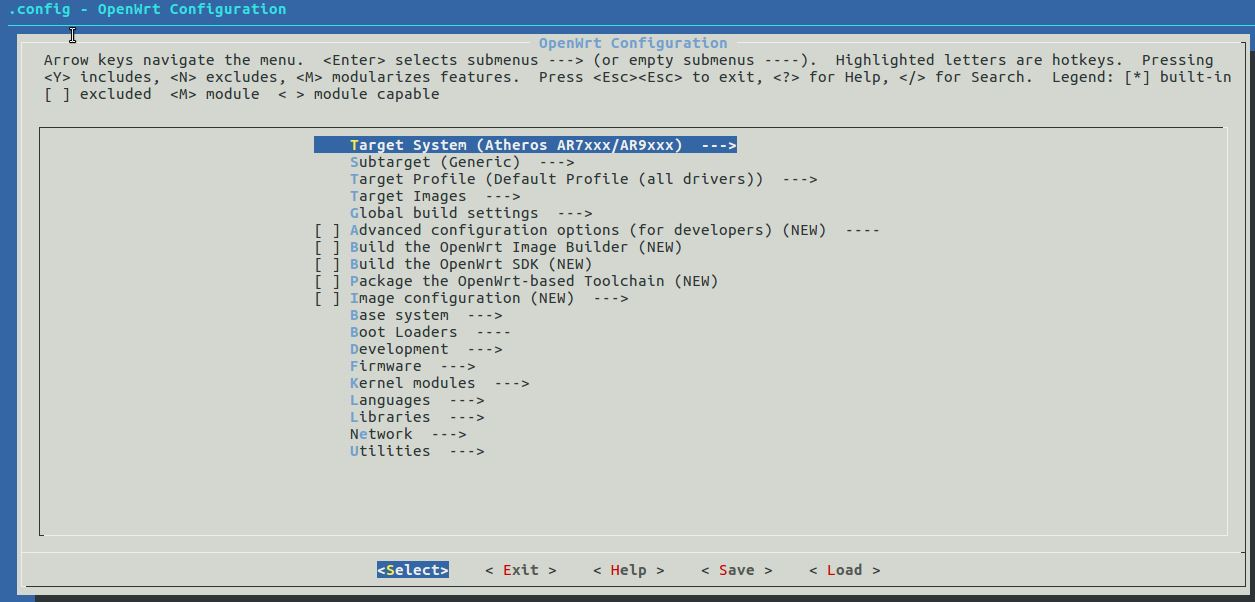
\includegraphics[width=\columnwidth]{image/menuconfig1.jpg}%
\caption{Menuconfig interface}%
\label{figure:menuconfig1}%-
\end{figure}

We are going to change a few things with this menu: the target system, the target profile, and the SDK.
First, we are going to put the target system to its right walue. In our case, we are using a GL-AR150. Therefore, we need to put:
\begin{lstlisting}[language=bash]
  'Atheros AR71xxx/AR9xxx'
\end{lstlisting}

If you are using a different router, you may have to choose another option.

Then, we are going to select GL-AR150 in the target profile.

Finally, we want to tick the box for 'Build the LEDE SDK' (or openwrt if your router is not using LEDE as an os).

We know save these changes and exit the menuconfig.

Now, we can finally build the SDK using the command:
\begin{lstlisting}[language=bash]
	###: make
\end{lstlisting}

This command may take a long time depending the power of your computer. For instance, on my Linux virtual machine (with 4GB of RAM and a laptop cpu) it took several hours to finish.

Once done, you will have a lot of new files. We are only interested in one repository:
\begin{lstlisting}[language=bash]
	staging_dir/toolchain-mips_24kc_gcc-5.4.0_musl-1.1.16
\end{lstlisting}

The name of the directory may change a bit but it will always start by toolchain.
So if you go to the 'bin' directory inside the toolchain, you should find the following file:
\begin{lstlisting}[language=bash]
	staging_dir/toolchain...bin/mips-openwrt-linux-musl-gcc
\end{lstlisting}

This executable is a c compiler for our router. We can use it on the linux computer to compile a c file. It will create an executable that can run on the router.


We know have our compiler. To use it we need to do the following steps:
\begin{itemize}
	\item export the bin directory in the PATH environment variable
	\item export a new environment variable called STAGING\_DIR (it will be used by the compiler
	\item precise to the makefile of the server where to find the compiler
\end{itemize}

Let's start by creating the environment variables. In your main repository, there is a file called .bashrc. This file is executed each time you start a shell. We are going to add two lines at the end of this file:
\begin{lstlisting}[language=bash]
	PATH=$PATH:~/staging_dir/toolchain.../bin/
	export STAGING_DIR=~/staging_dir/toolchain.../
\end{lstlisting}

Now we only need to slightly change the makefile. Go to the repository containing the sources.
In the makefile, there is at the top of the file a variable called SERVERCC.
This variable precise the compiler used for the server.c file.
To compile it for the router, we just need to change its value to the correct gcc: mips-openwrt-linux-musl-gcc
If we later want to compile the server.c file for the linux computer (to do some testing), we only need to change back this variable to gcc.


Now we can create the server exec file by doing:

\begin{lstlisting}[language=bash]
	###: make server
\end{lstlisting}

\large WARNING:\\
The server and the client have two mode DEBUG and normal. To change the mode of functioning, you have to change the value of a line in their respective c files. The line to change is:
\begin{lstlisting}[language=c]
	#define DEBUG 1
\end{lstlisting}
If the value of this line is 0, it means you are in DEBUG mode. Make sure to put any other number than 0 before doing make.

\subsubsection{Adding the server to the router}

We now have an executable called 'server'. In this part, we will:
\begin{itemize}
	\item add this file to the router
	\item automatize its start
\end{itemize}



To add the file to the router, we just use scp (which is a copy function over a ssh connection) to copy the executable anywhere in the router.


Now we are going to automatize the server. We want two things:
\begin{itemize}
	\item the server start during the boot
	\item if the server crash, a script is launching it again
\end{itemize}

First, let's start by writing the script that will start the server at the boot:


\begin{lstlisting}
#!/bin/sh /etc/rc.common

# The order you want these scripts to be run. 
# e.g Start=6 will run after scripts with Start=5 but before Start=7
START=6
STOP=12

# The command(s) you want to run on start
start() {        
        echo starting
	PATH_of_server_executable
}                 

# The command(s) you want to run on stop
stop() {          
        echo stopping
				
}
\end{lstlisting}



Now we want to restart the server if he crash.
To do achieve that, we are going to use crontab and the following script.

\begin{lstlisting}
	#!/bin/sh
	result=`netstat -an|grep 8800| grep LISTEN`
	if [ -z "$result" ]
	then
		/path_to_server
	fi
\end{lstlisting}



We will execute this script every 10 minutes.
By default cron is disable on lede. We can enable it with the following command:
\begin{lstlisting}
	/etd/init.d/cron enable
\end{lstlisting}

We can now run cron:
\begin{lstlisting}
	crontab -e
\end{lstlisting}


It will open a file with vi. On this file we want to add the following line
\begin{lstlisting}
*/10 * * * * path_to_script
\end{lstlisting}



If you want to adjust how often it repeat, here is how crontab work. The line is composed of the following elements
minute hour day(month) year day(week) command\_to\_execute

For the first 5 value, there are special characters:
\begin{itemize}
	\item * represents any value
	\item , is a value line separator
	\item / is used for step values
	\item - is a range of value
\end{itemize} 

